\section{Data Analysis}
Our data set consisted of the daily open, high, low, and close (OHLC) values for the time period 1999-01-01 through 2019-12-31 of the following major currency pairs
\begin{itemize}
    \item EURUSD - Euro € / U.S. Dollar \$
    \item GBPUSD - British Pound Sterling £ / U.S. Dollar \$
    \item USDCAD - U.S. Dollar \$ / Canadian Dollar \$
    \item USDJPY - U.S. Dollar \$ / Japanese Yen ¥
\end{itemize}
obtained from Dukascopy historical data feed~\cite{dukascopy}.
The data set was filtered to remove days where any of the currencies had zero volume, as well as NYSE and LSE holidays.
This resulted in a data set of 5165 training samples.
Here we use the notation \( x_\text{open} \), \( x_\text{high} \), \( x_\text{low} \), and \( x_\text{close} \) to denote the open, high, low, and close values of a currency pair on a particular day.

Given that the values were on an absolute basis, we needed to convert them to relative terms in order to be able to compare data from different time periods on a more equal footing.
The natural way to do so was to compare the returns
\begin{align}
    r = \frac{x_\text{close} - x_\text{open}}{x_\text{open}}.
\end{align}
However, this wasn't necessarily the best way to approach this.
Instead we opted to use the log returns
\begin{align}
    \tilde{r}
        = \log(1+r)
        = \log\bigg( \frac{x_\text{close}}{x_\text{open}} \bigg)
\end{align}
due to several advantages~\cite{quantivity_2012}
\begin{itemize}
    \item Log-normality: if \( r \sim \mathcal{N}(\mu, \sigma^2) \) then \( \tilde{r} \sim \mathcal{N}(\tilde{\mu}, \tilde{\sigma}^2) \).
    \item Small \( r \) approximation: the expansion \( \log (1 + r) = r + \mathcal{O}(r^2) \approx r \) for \( r \ll 1 \).
    \item Time-additivity: instead of having to multiply one plus the returns to compound them, using log returns allows one to simply add them.
\end{itemize}

We began our analysis by taking a look at the histograms depicted in~\cref{fig:histograms_raw}.
From visual examination we saw that the log returns were roughly normally distributed with the statistics given in~\cref{tbl:data_log_returns_raw_stats}.
\begin{figure}[!htb]
    \begin{center}
        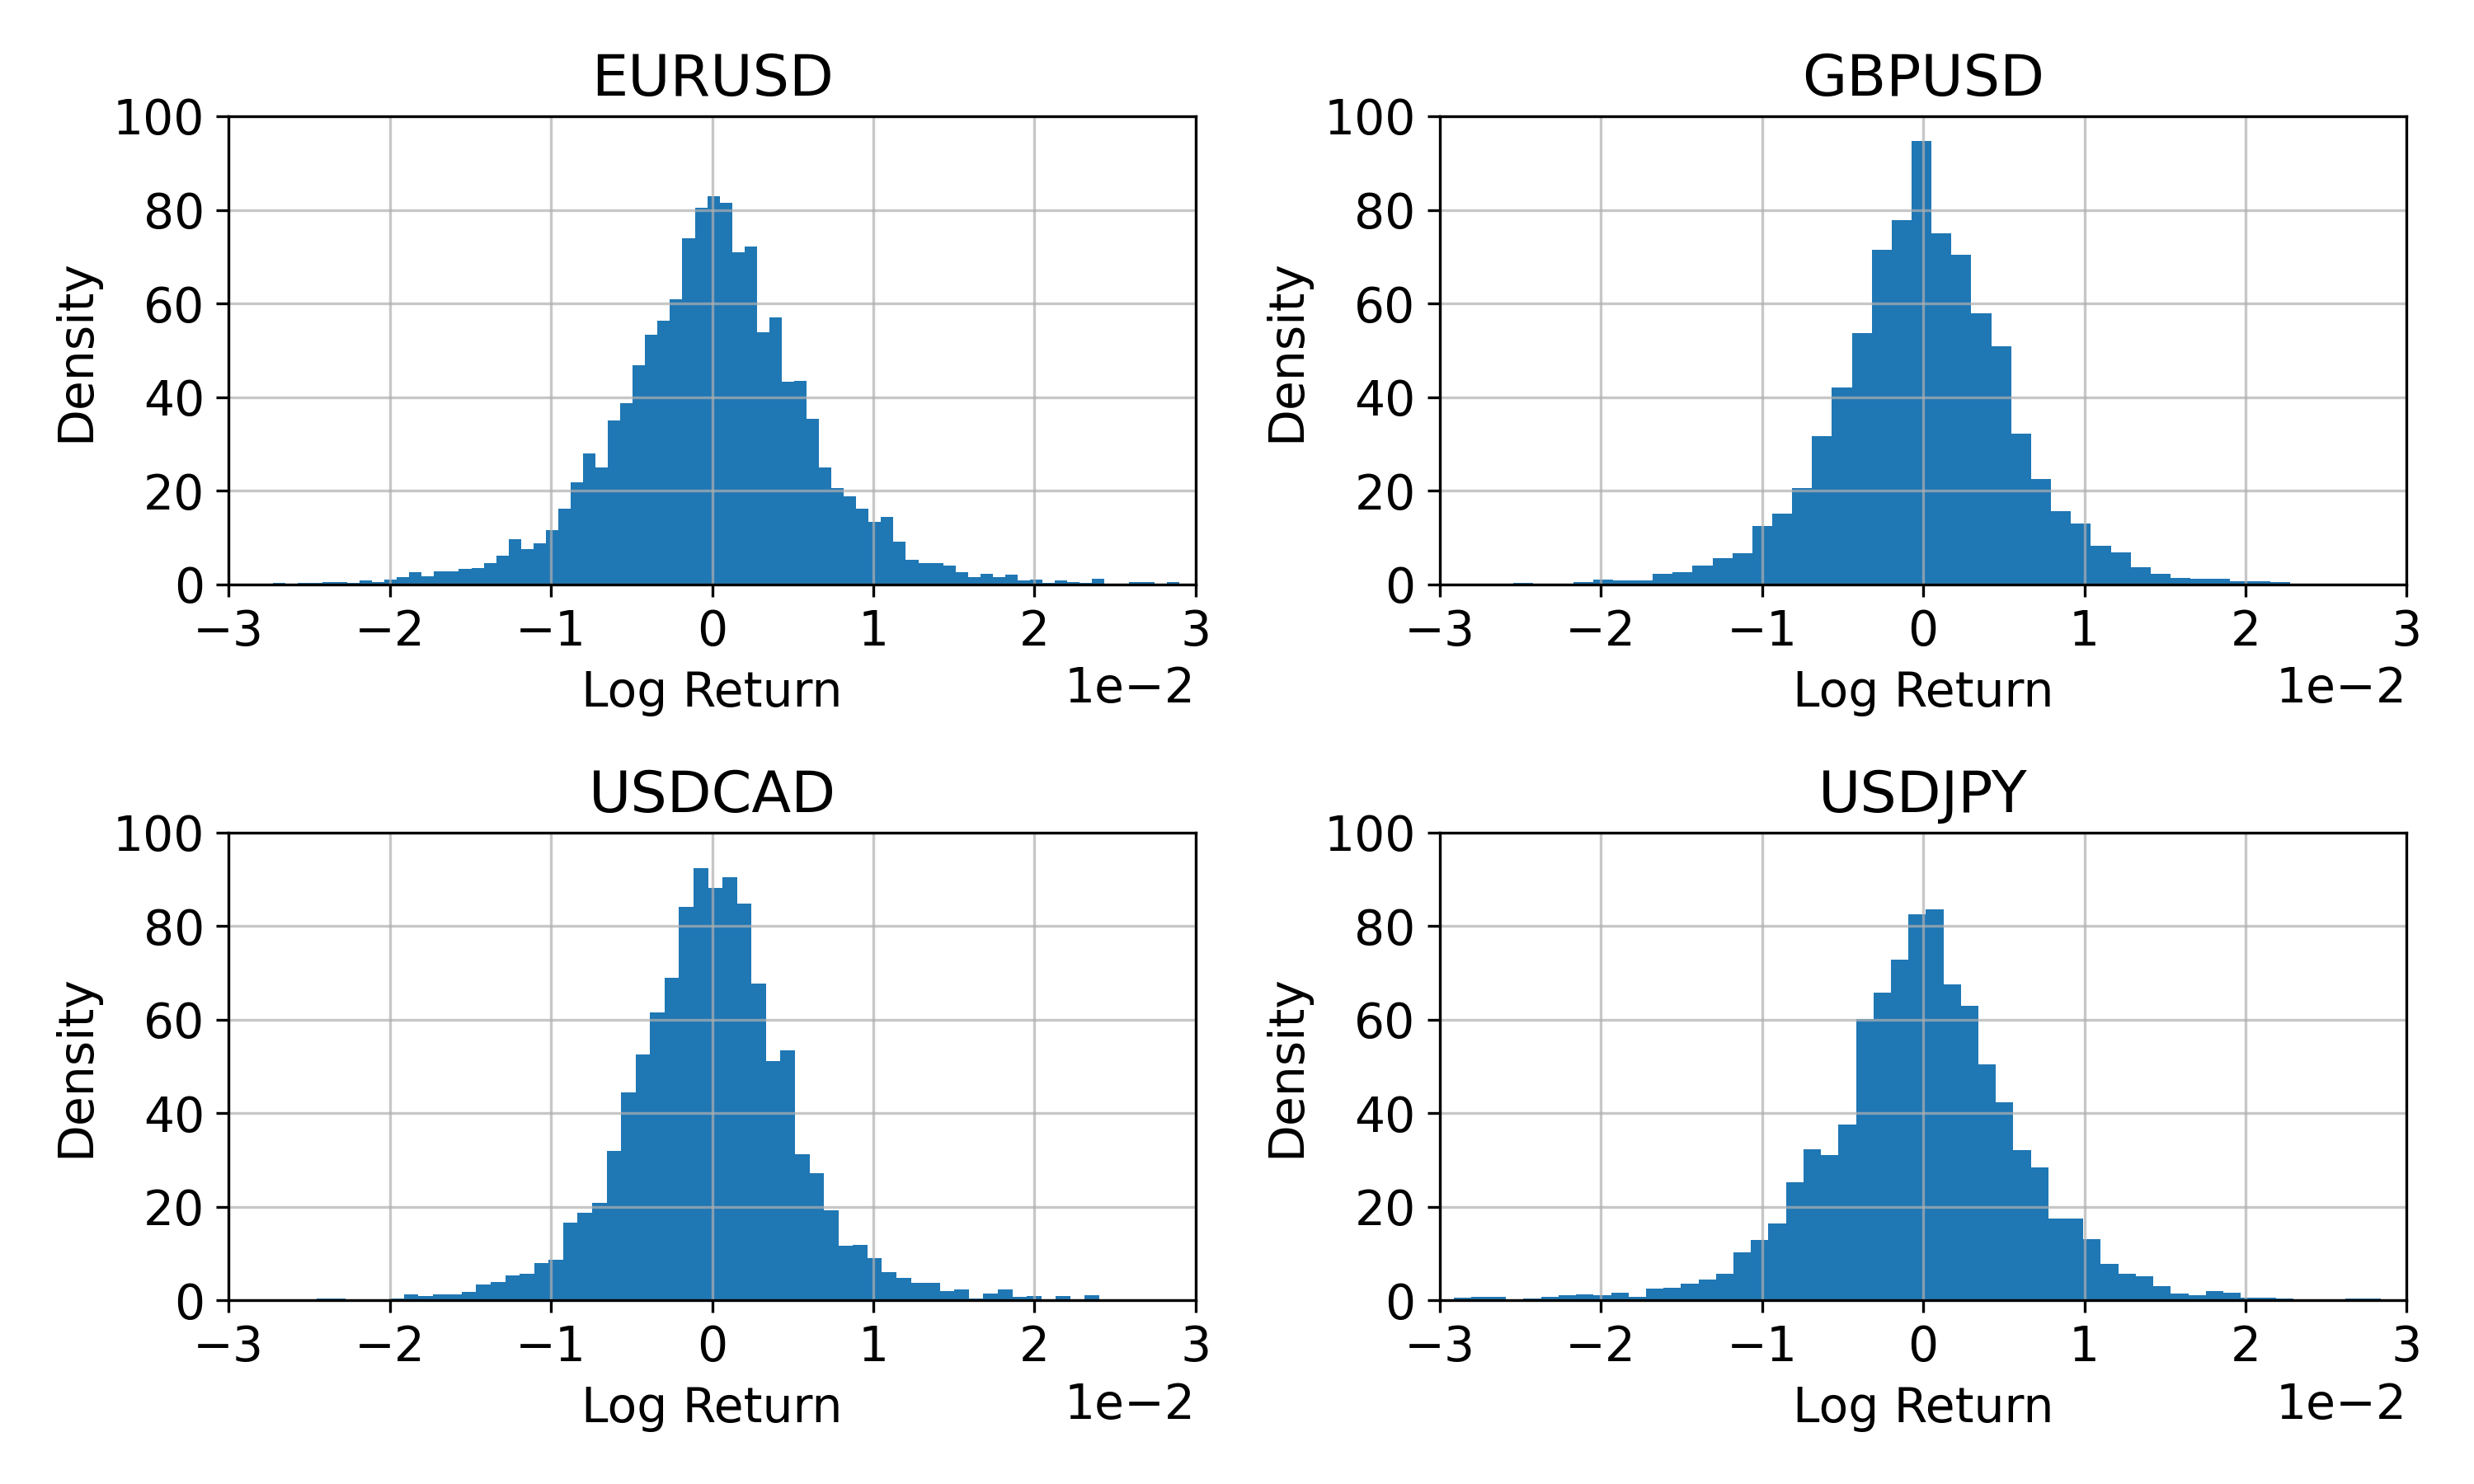
\includegraphics[width=1\linewidth]{data_analysis/histograms.png}
    \end{center}
    \caption{Histograms of the log returns data set.}
    \label{fig:histograms_raw}
\end{figure}

\begin{table}[!htb]
    \centering
    \begin{adjustbox}{max width=\textwidth}
        \input{../tables/data/log_returns_raw_stats.tbl}
    \end{adjustbox}
    \caption{Statistics of the log returns data set.}
    \label{tbl:data_log_returns_raw_stats}
\end{table}

We also visualized the log returns in a violin and box plot in~\cref{fig:violin_raw}, which allowed us to identify outliers and see how they were distributed.
Immediately we saw that there was one major outlier to the downside for the GBPUSD currency pair.
Further analysis indicated that this was an \( 11.1\sigma \) event that occurred on 2016-06-24, which corresponded to the results of the Brexit referendum in the UK~\cite{brexit_gov_uk}.
The other outlier that really stood out was to the upside for the USDJPY currency pair on 2008-10-28.
This \( 8.3\sigma \) event occurred right in midst of the financial crisis when people were talking about the end of the Yen carry trade~\cite{jpy_carry_trade_nyt}.
In the final training data set we chose to remove outliers greater than \( 10\sigma \) from the mean.
\begin{figure}[!htb]
    \begin{center}
        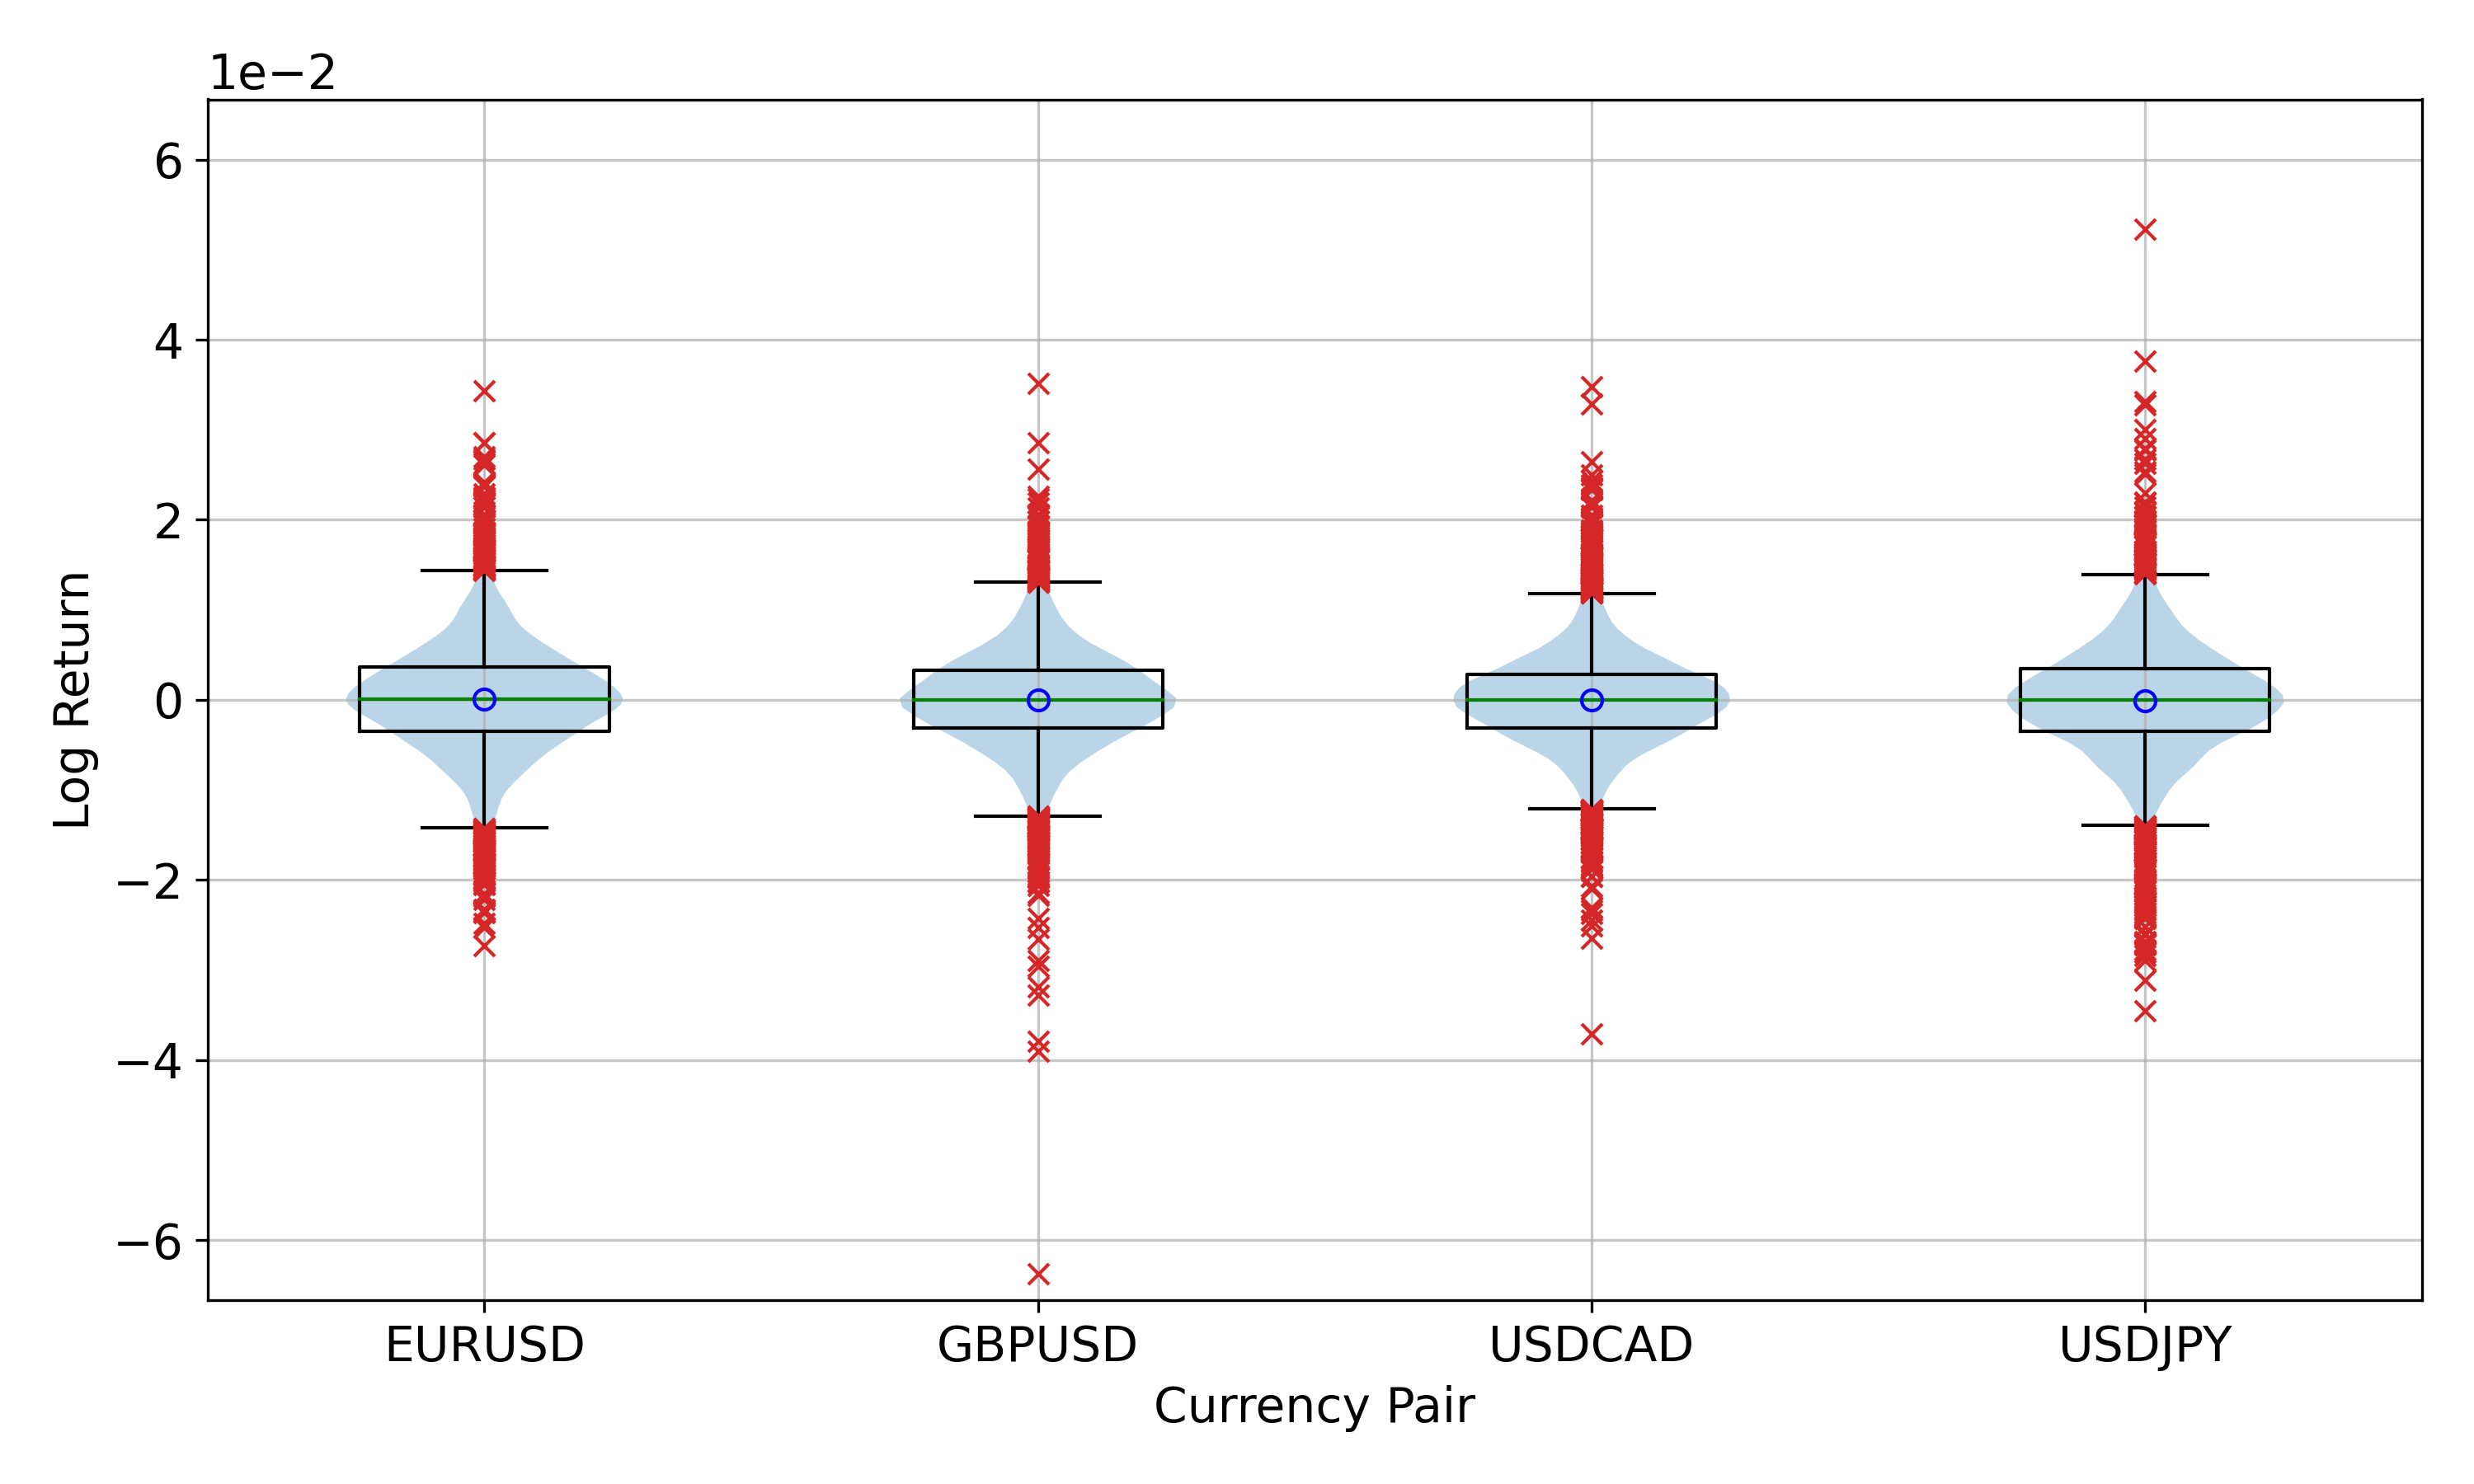
\includegraphics[width=1\linewidth]{data_analysis/violin.png}
    \end{center}
    \caption{Violin and box plot of the log returns data set illustrating the distribution of the outliers.}
    \label{fig:violin_raw}
\end{figure}

Next we examined the correlations between the currency pairs to get an idea of the interdependencies between them.
We visualized this with scatter plots in~\cref{fig:scatters} where we observed a clear positive correlation between EURUSD/GBPUSD, and clear negative correlations between EURUSD/USDCAD and GBPUSD/USDCAD.
We verified this by examining the Pearson \( r \), Spearman \( \rho \), and Kendall \( \tau \) correlation coefficients laid out in~\cref{tbl:data_correlation_coefficients}.
We found the correlation coefficients to be positive when the pairs were of the form \( X \)USD/\( Y \)USD, and negative when the pairs were of the form \( X \)USD/USD\( Y \), for \( X,Y \in \) \{EUR, GBP, CAD, JPY\}, as expected.
Details on how the correlation coefficients were computed and how to interpret them can be found in~\cref{app:correlation_coefficients}.
\begin{figure}[!htb]
    \begin{center}
        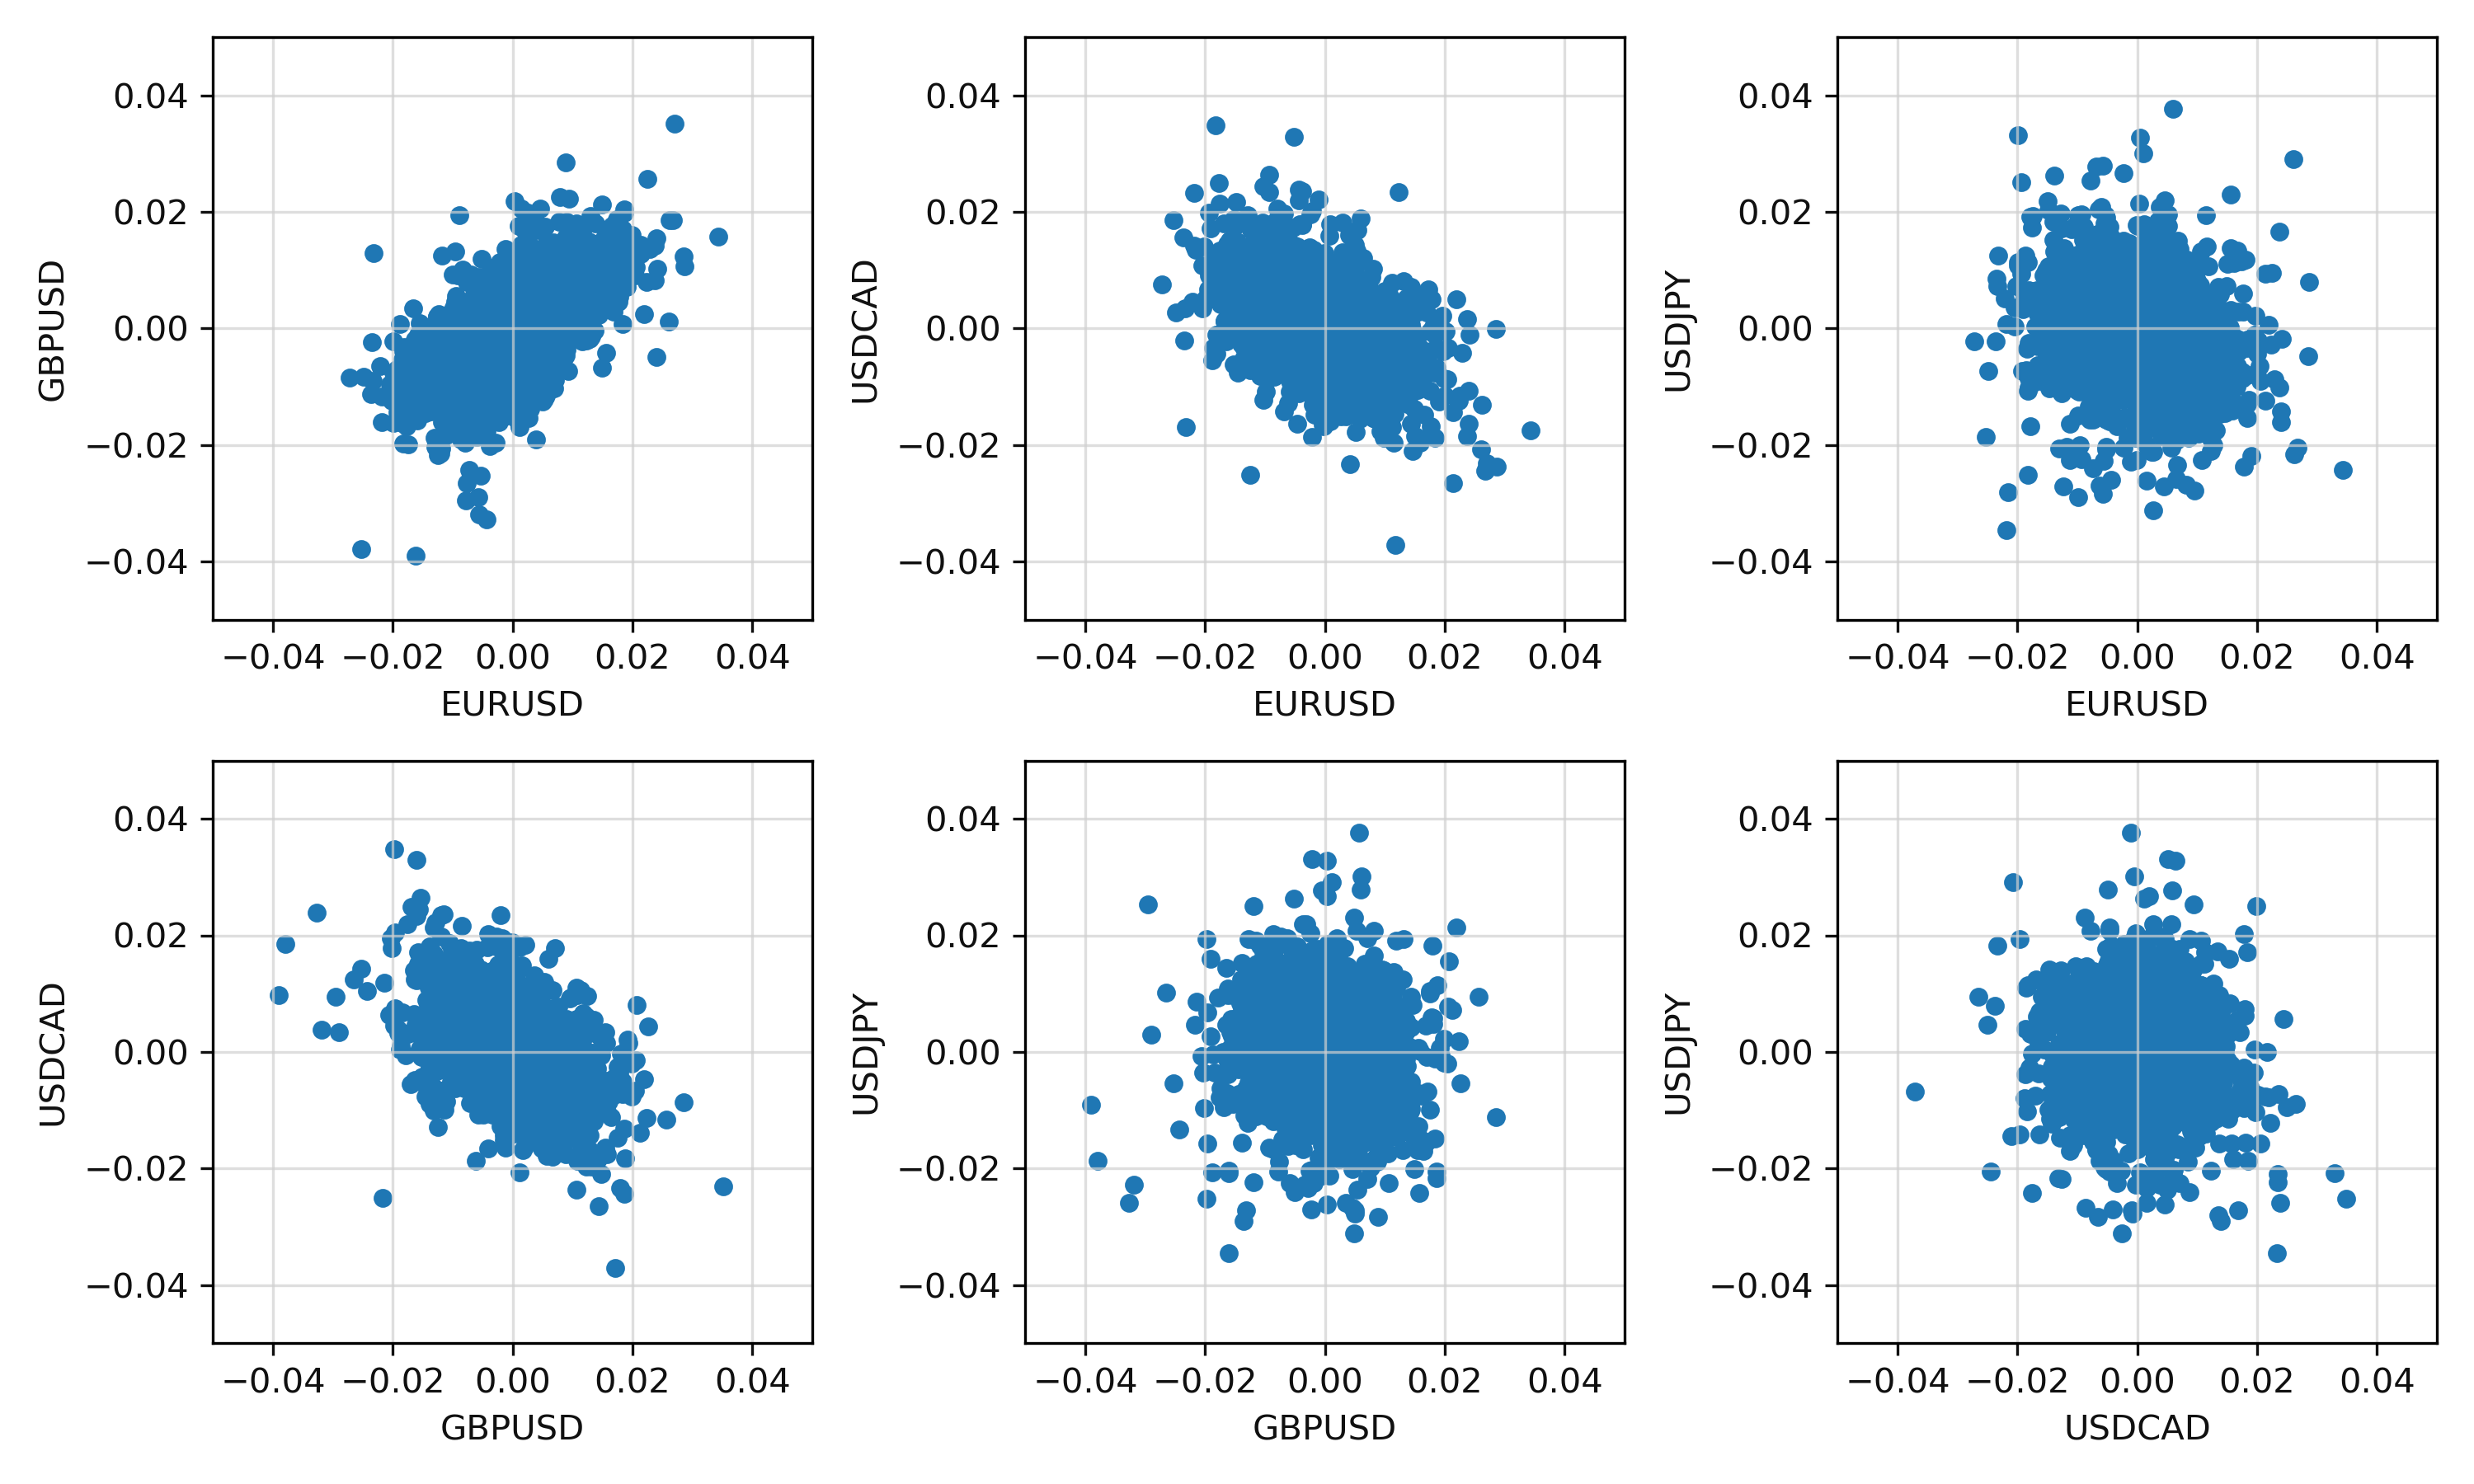
\includegraphics[width=1\linewidth]{data_analysis/scatters.png}
    \end{center}
    \caption{Scatter plots of the log returns data set.}
    \label{fig:scatters}
\end{figure}

\begin{table}[!htb]
    \centering
    \begin{adjustbox}{max width=\textwidth}
        \input{../tables/data/correlation_coefficients.tbl}
    \end{adjustbox}
    \caption{Correlation coefficients of the log returns data set.}
    \label{tbl:data_correlation_coefficients}
\end{table}


\section{Data Preprocessing}
The models used in this thesis required the training data to be in the form of bit vectors, so we had to first convert our data set to such a form.
Let \( \mat{X} \in \R^{4 \times N} \) represent the training data set of log returns with \( N \) samples, where training samples are vectors in the column space, thus element \( x_{ij} \) represents the \( i \)th currency pair log return for the \( j \)th training sample.

To discretize the data, we rescaled and rounded the entries of \( \mat{X} \) to integer values in \( \{0, 1, \dots, 2^{n_\text{bits}} - 1\} \), represented by the matrix \( \mat{X}' \in \N^{4 \times N} \) with entries
\begin{align}
    x_{ij}' = \bigg\lfloor \frac{x_{ij} - \min_k \{x_{ik}\}}{\max_k \{x_{ik}\} - \min_k \{x_{ik}\}} \cdot (2^{n_\text{bits}} - 1) \bigg\rceil,
\end{align}
where \( \lfloor \ \cdot \ \rceil \) denotes rounding to the nearest integer.

A new matrix \( \mat{V} \in \binset^{4\cdot n_\text{bits} \times N} \) was then created with the columns being the \( n_\text{bits} \)-length bit vectors corresponding to the binary representation of the entries of the columns of \( \mat{X}' \) concatenated together.
For example, if \( \vec{x}' = (x_1',x_2',x_3',x_4') \) was a column of \( \mat{X}' \) and the function \( \text{bitvector}(x') \) takes in an integer \( x' \) and returns an \( n_\text{bits} \)-bit binary representation bit vector, then the corresponding column in \( \mat{V} \) would be
\begin{align}
    \vec{v} = \begin{bmatrix}
        \text{bitvector}(x_1') \\
        \text{bitvector}(x_2') \\
        \text{bitvector}(x_3') \\
        \text{bitvector}(x_4') \\
    \end{bmatrix}
    \in \binset^{4\cdot n_\text{bits}}.
\end{align}

For this research we took \( n_\text{bits} = 16 \), which gave us a training set \( \mat{V} \in \binset^{64 \times N} \), thus our training samples were bit vectors of length 64.
The discretization errors associated with this conversion and data set were on the order of \( 10^{-7} \), well within the desired tolerance for this purpose.

\subsection{Data Transformation}\label{sec:outlier_transform}
Due to how the data was linearly converted to a discrete form before rounding, it opened up the possibility of the discretized data being clustered in the mid-range values if large outliers were present.
To mitigate this, we came up with a transformation to reduce the gap between outliers by scaling outliers beyond a certain threshold \( \tau \), as detailed in~\cref{alg:transformation}.
We call this the outlier power transformation.
In practice we took \( \tau = 1 \) and \( \alpha = 0.5 \), thus the standardized data points above one standard deviation were mapped to their square root, as illustrated in~\cref{fig:data_transformation}.
We did explore a few other combinations of \( \tau \) and \( \alpha \), but found these values to produce the best results out of those we tried; of course this could likely be further optimized.
This transformation is invertible when \( \overline{x} \), \( \sigma_x \), and \( \delta \) are saved.

\begin{algorithm}
\caption{Outlier Power Transformation}
\begin{algorithmic}[1]
    \Procedure{Transform}{$\vec{x}, \alpha, \tau$}
            \Comment $\alpha$ is the power, $\tau$ is the threshold
        \State $\overline{x} \gets \text{mean}(\vec{x})$
        \State $\sigma_{x} \gets \text{std}(\vec{x})$
        \State $\delta \gets \tau - \tau^\alpha$
            \Comment ensures the transformation is bijective
        \For {$i$ in 1 to length($\vec{x}$)}
            \State $x_i \gets (x_i - \overline{x}) / \sigma_x$
                \Comment standardize
            \If {$x_i > \tau$}
                \State $x_i \gets (\abs{x_i}^\alpha + \delta) \cdot \text{sign}(x_i)$
                    \Comment scale standardized values beyond $\tau$
            \EndIf
            \State $x_i \gets x_i \cdot \sigma_x + \overline{x}$
                \Comment undo standardization
        \EndFor
    \EndProcedure
\end{algorithmic}
\label{alg:transformation}
\end{algorithm}

\begin{figure}[!htb]
    \begin{center}
        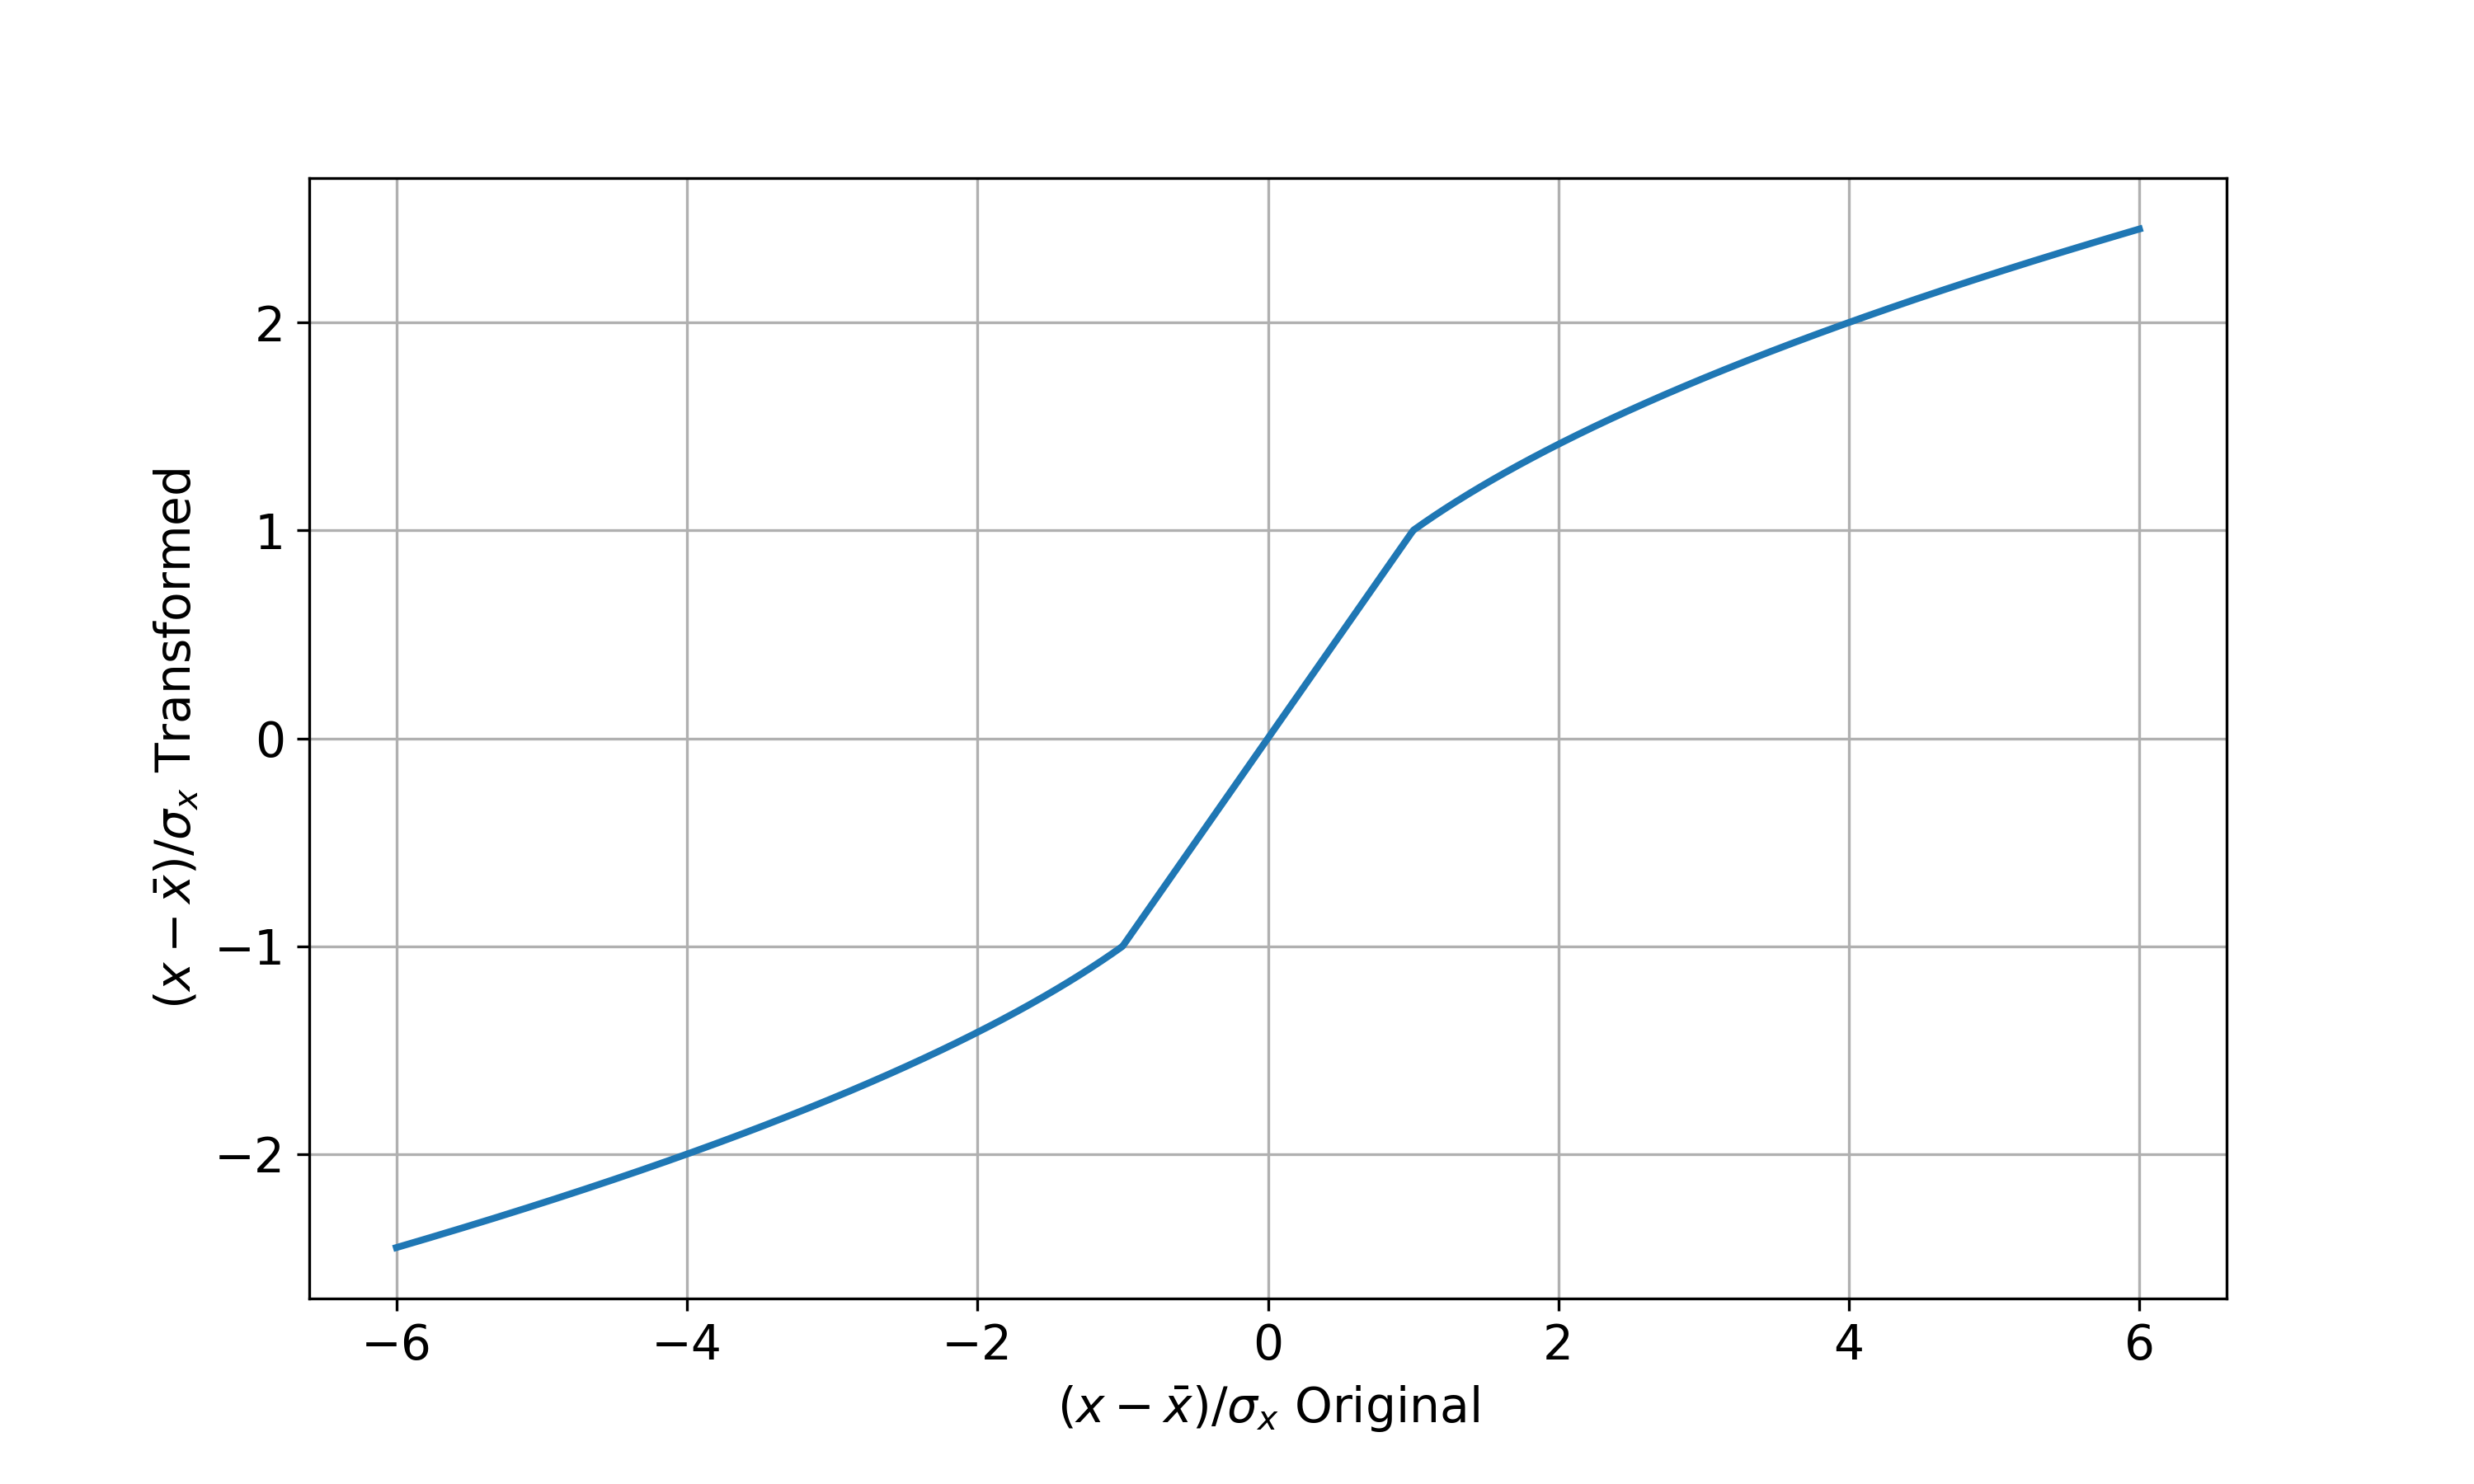
\includegraphics[width=1\linewidth]{data_analysis/data_transformation.png}
    \end{center}
    \caption{Transformation defined in~\cref{alg:transformation} using \( \tau = 1 \) and \( \alpha = 0.5 \), for the purpose of reducing large gaps in the discretized data set by scaling outliers above \( \tau \) standard deviations.}
    \label{fig:data_transformation}
\end{figure}

We visualized the transformed data set with histograms in~\cref{fig:data_transformation} and a violin and box plot in~\cref{fig:violin_transformed}.
In these, we observed the appearance of "shoulders" around one standard deviation where the outliers were scaled in, and that the outliers became much less extreme, allowing us to better utilize the full range of discrete values.
\cref{tbl:data_log_returns_transformed_stats} shows that the standard deviations were decreased to roughly \( 78\% \) of their originals values in~\cref{tbl:data_log_returns_raw_stats}.

\begin{figure}[!htb]
    \begin{center}
        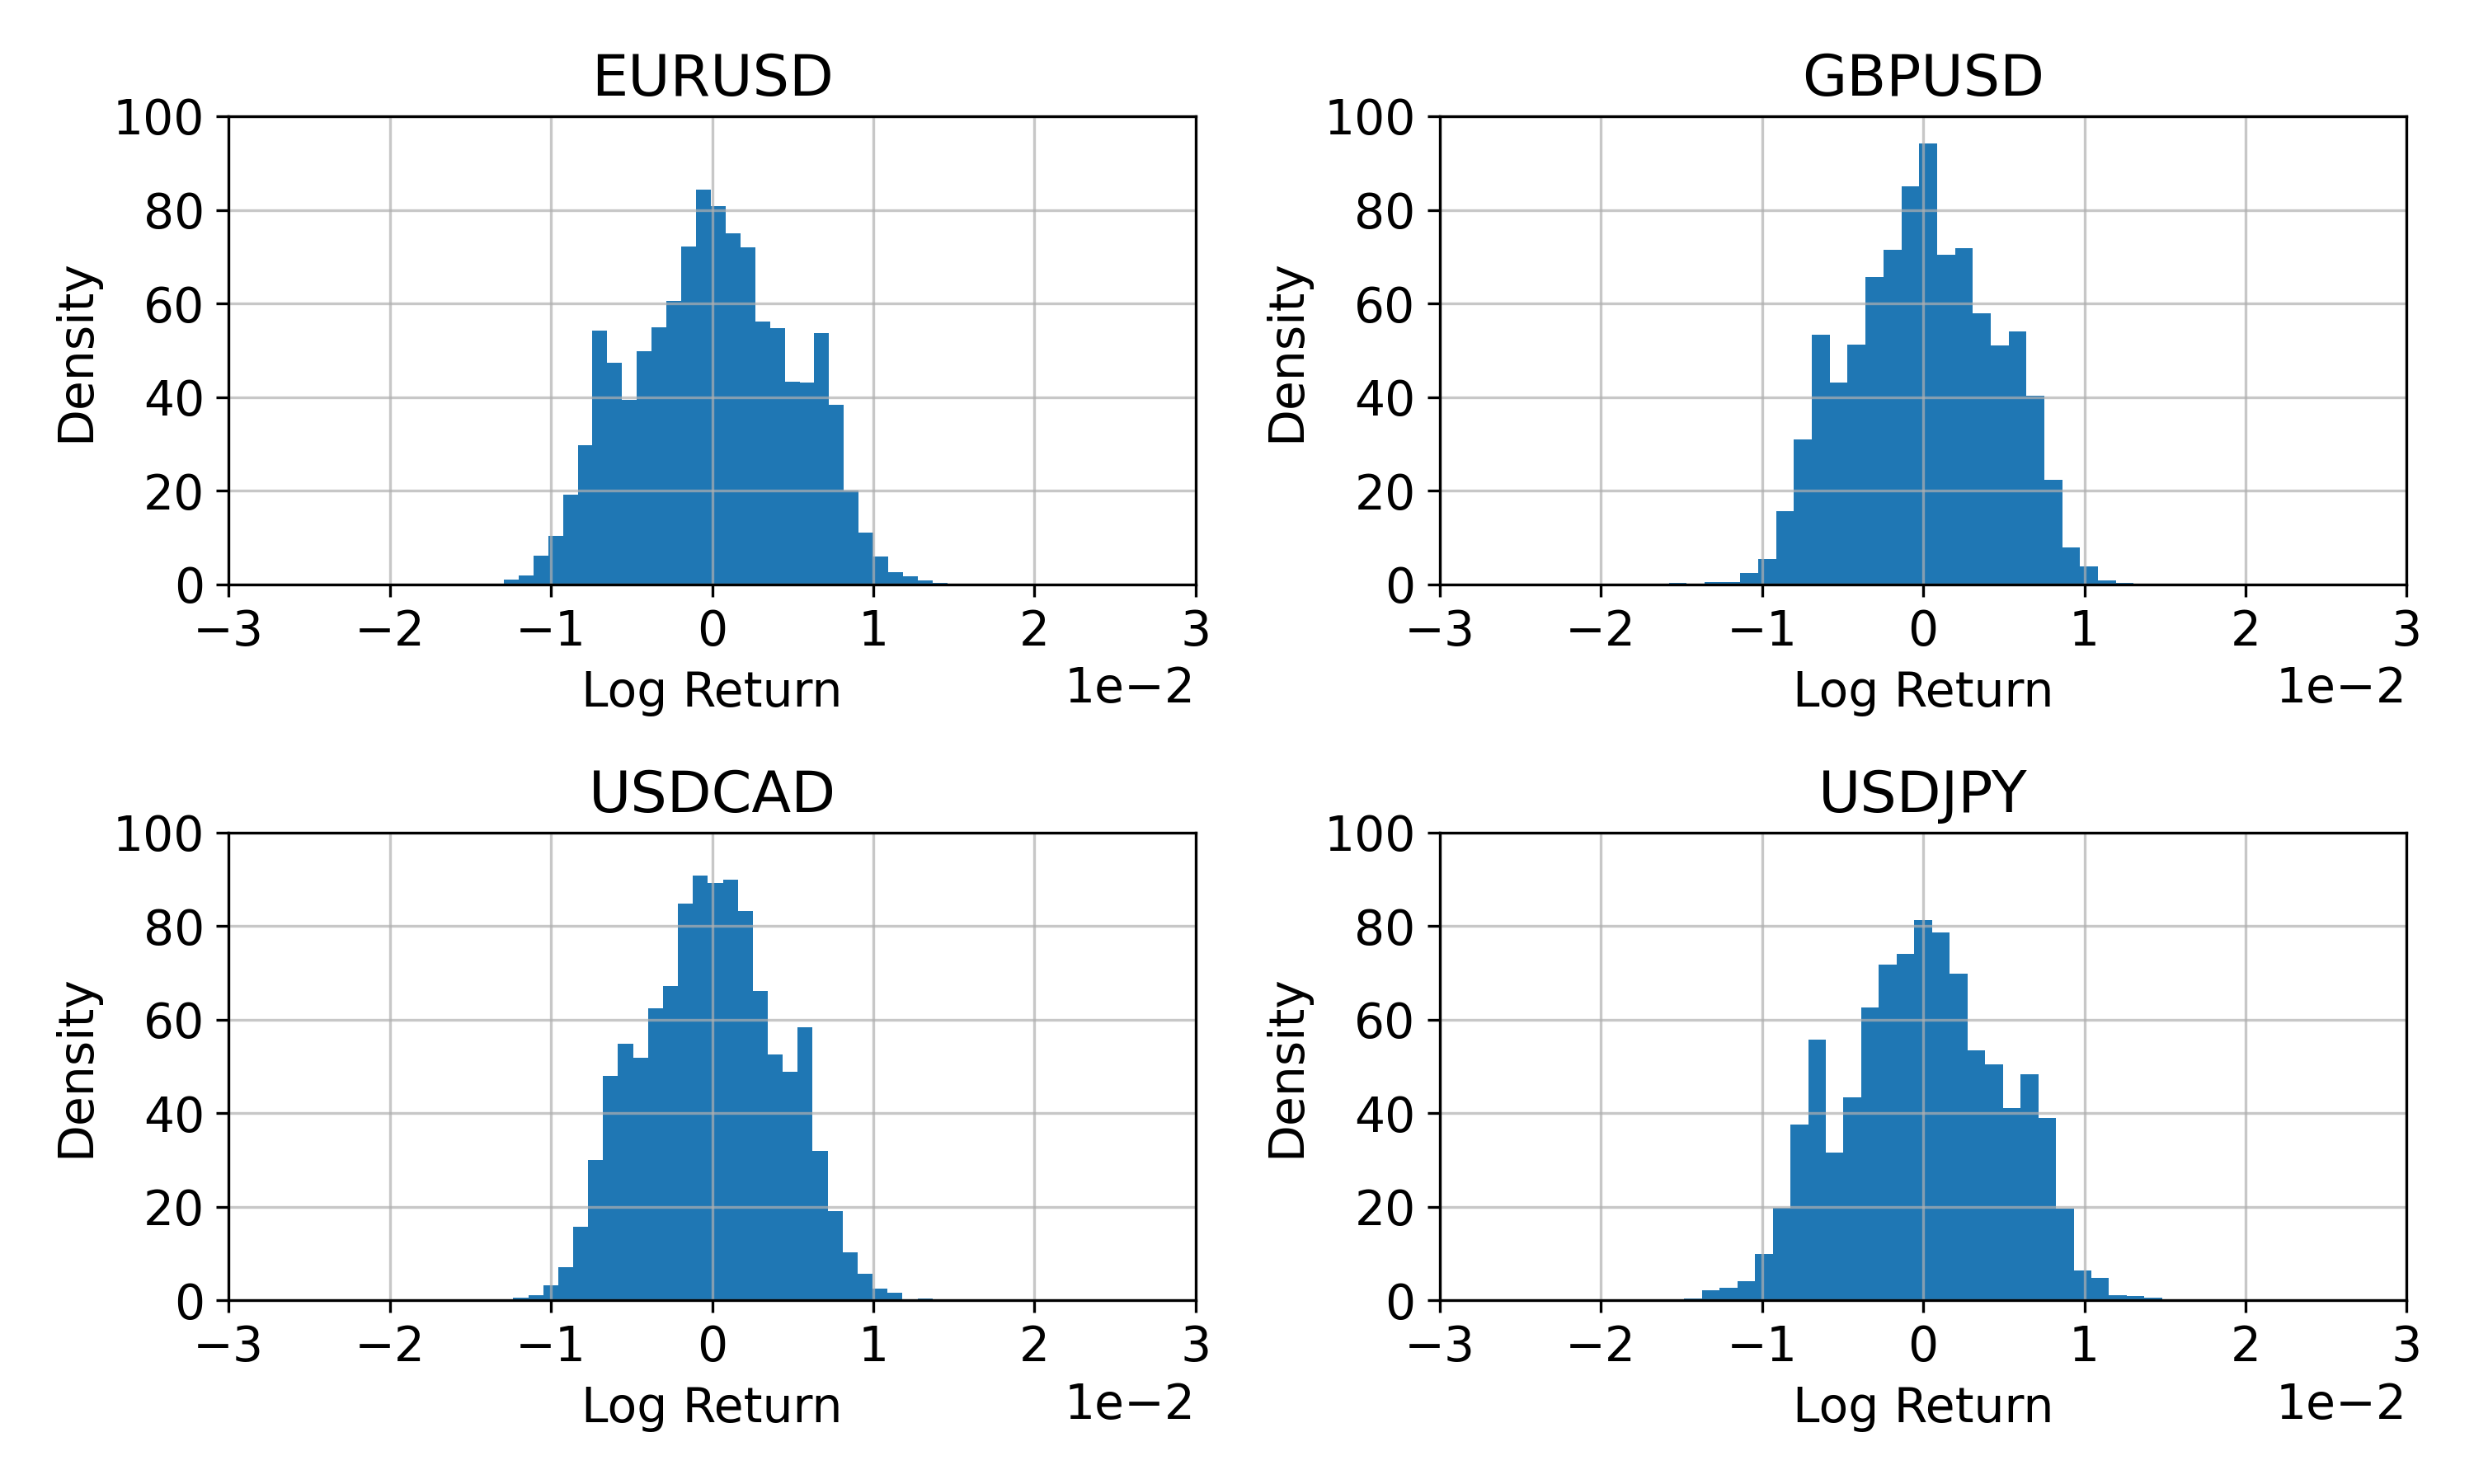
\includegraphics[width=1\linewidth]{data_analysis/histograms_transformed.png}
    \end{center}
    \caption{Histograms of the outlier power-transformed log returns data set.}
    \label{fig:histograms_transformed}
\end{figure}
\begin{figure}[!htb]
    \begin{center}
        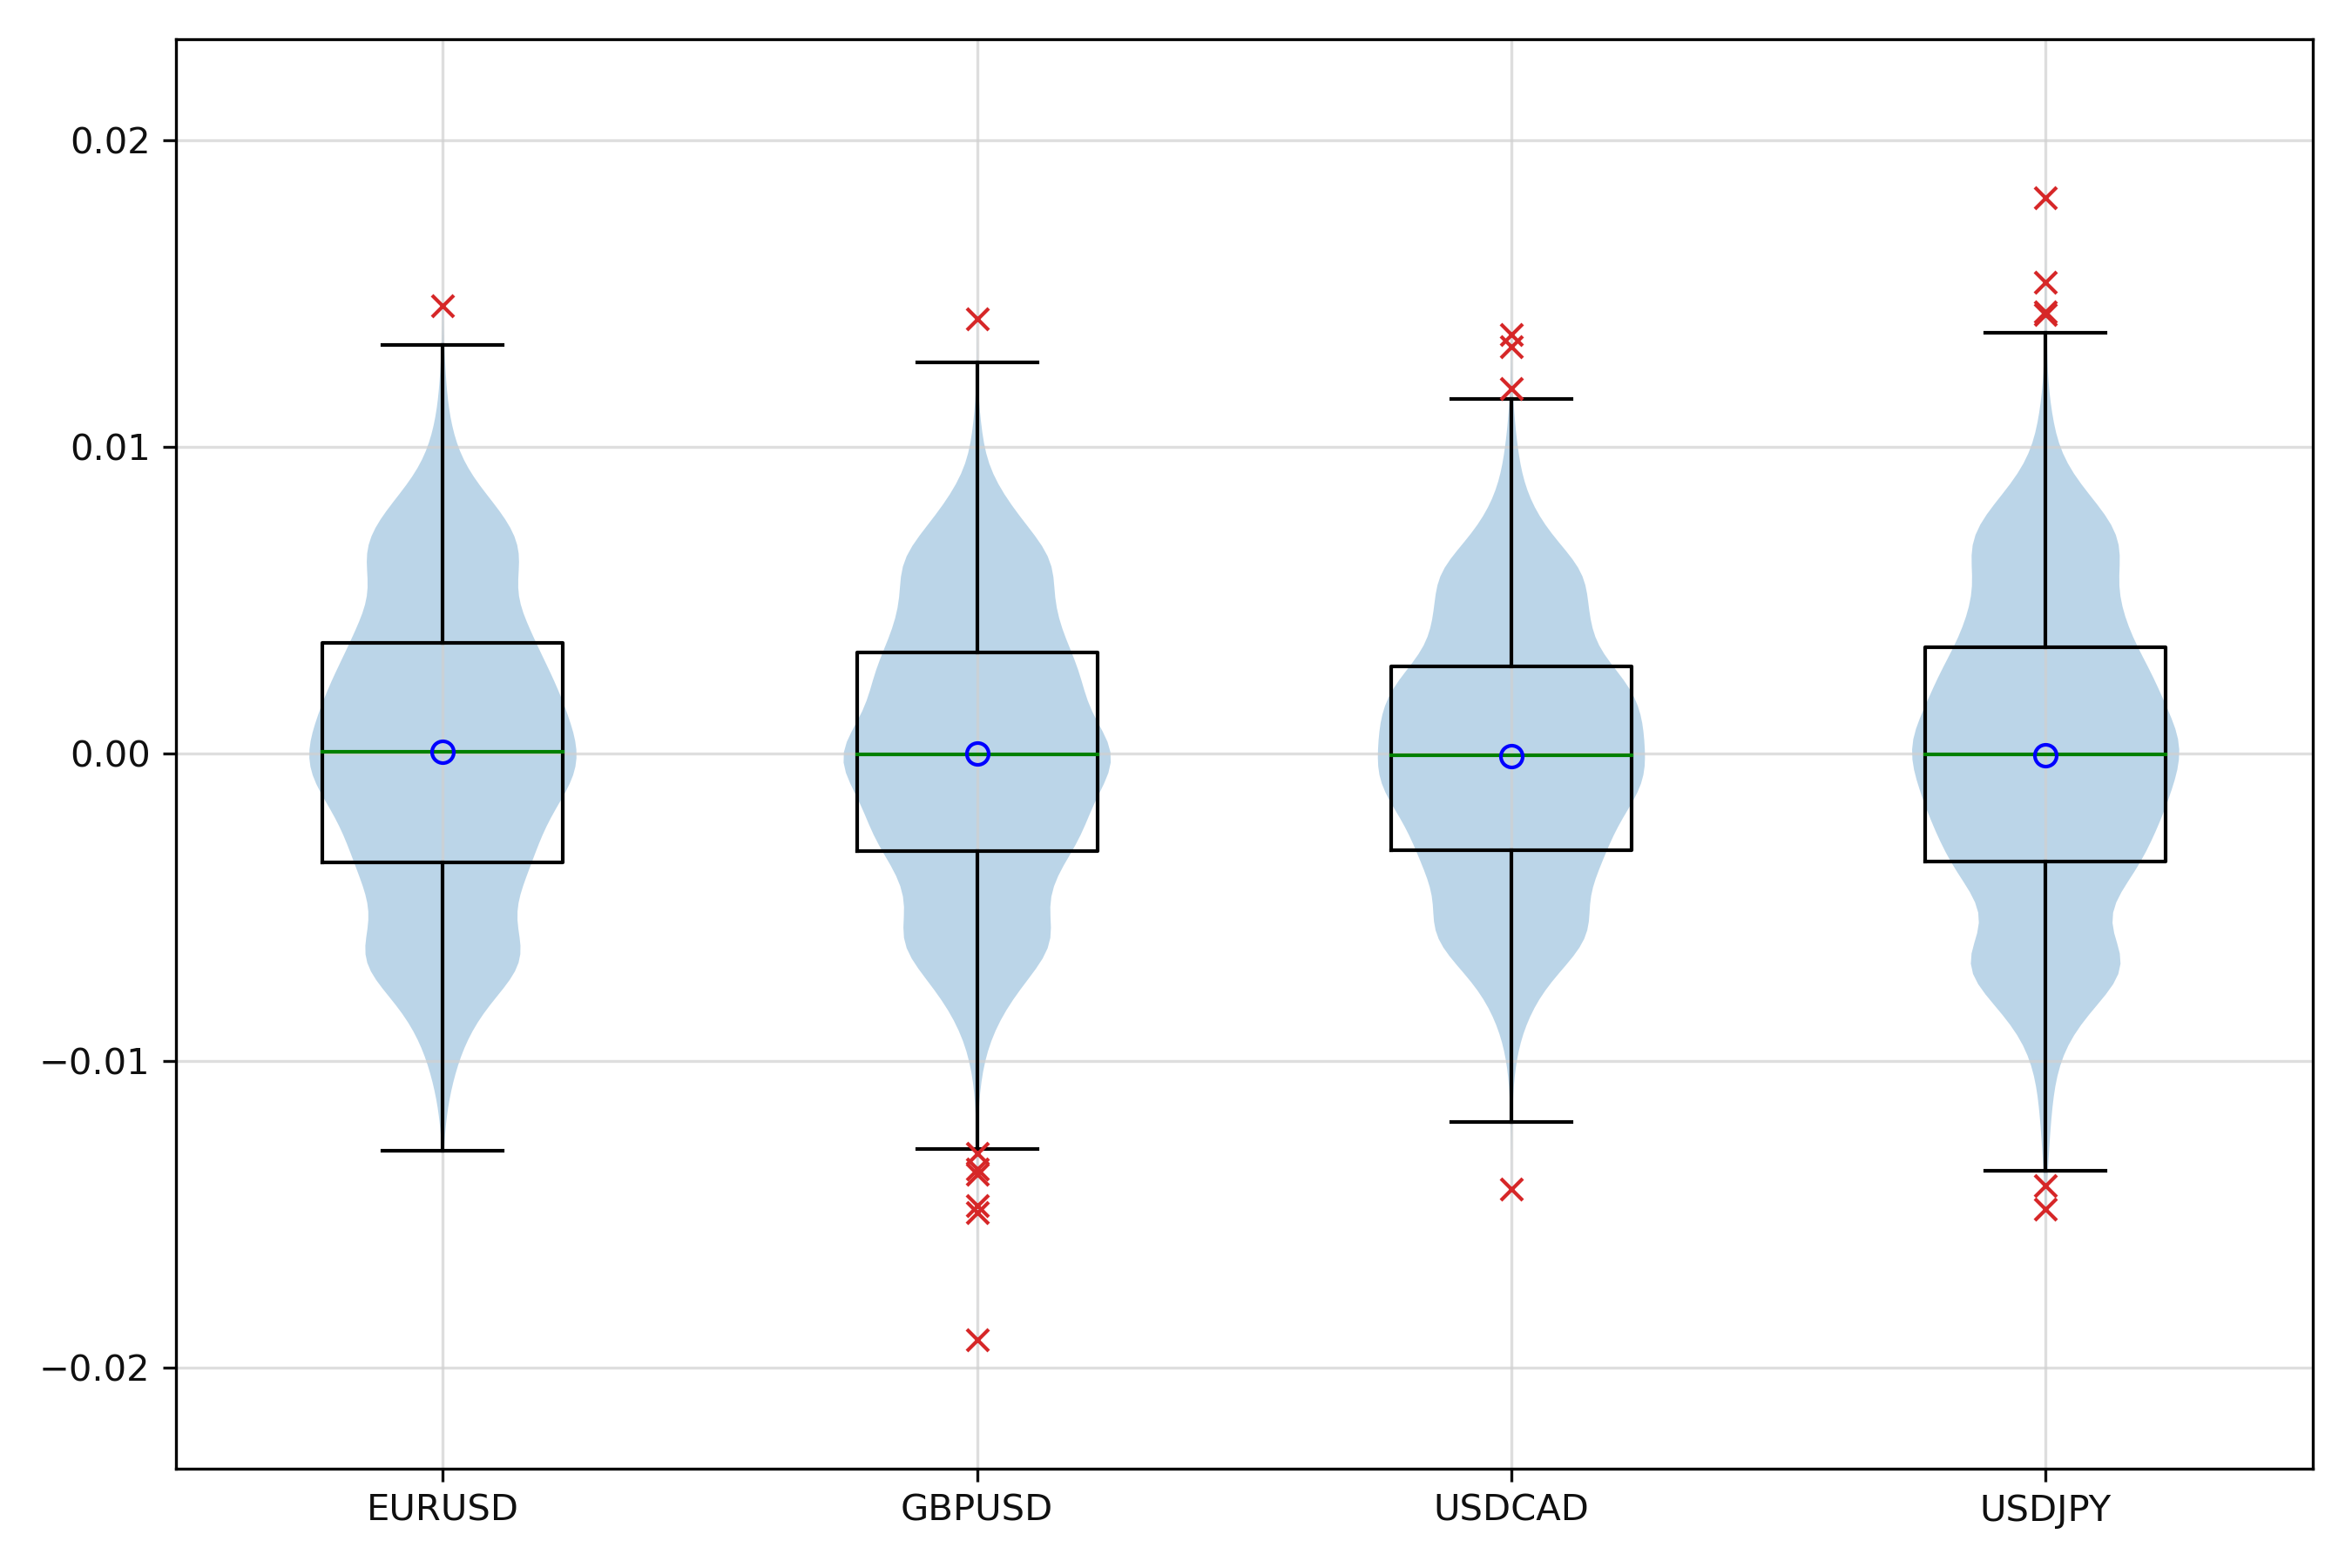
\includegraphics[width=1\linewidth]{data_analysis/violin_transformed.png}
    \end{center}
    \caption{Violin and box plot of the outlier power-transformed log returns data set illustrating the distribution of the rescaled outliers.}
    \label{fig:violin_transformed}
\end{figure}
\begin{table}[!htb]
    \centering
    \begin{adjustbox}{max width=\textwidth}
        \input{../tables/data/log_returns_transformed_stats.tbl}
    \end{adjustbox}
    \caption{Statistics of the outlier power-transformed log returns data set.}
    \label{tbl:data_log_returns_transformed_stats}
\end{table}

\subsection{Additional Information}
As mentioned in~\cite{kondratyev_2019}, one can use additional binary indicator variables to enrich the training data set.
One such bit of information is the rolling volatility relative to the historical median (see~\cref{app:annualized_volatility} for definition of annualized volatility).
If the 3-month rolling volatility was (below) above the historical median it was assigned a value of 0 (1) to indicate the low (high) volatility regime.
We plotted the 3-month rolling volatilities versus their historical medians in~\cref{fig:rolling_volatility}.

These additional binary indicator variables were then concatenated onto the training data set and fed to the model to make it more flexible by allowing for the model outputs to be conditioned on a specific volatility regime.
Adding one indicator for each of the four currency pairs increased the number of rows in our training data set by four, thus the concatenated data set was in the space \( \binset^{68 \times N} \).

\begin{figure}[!htb]
    \begin{center}
        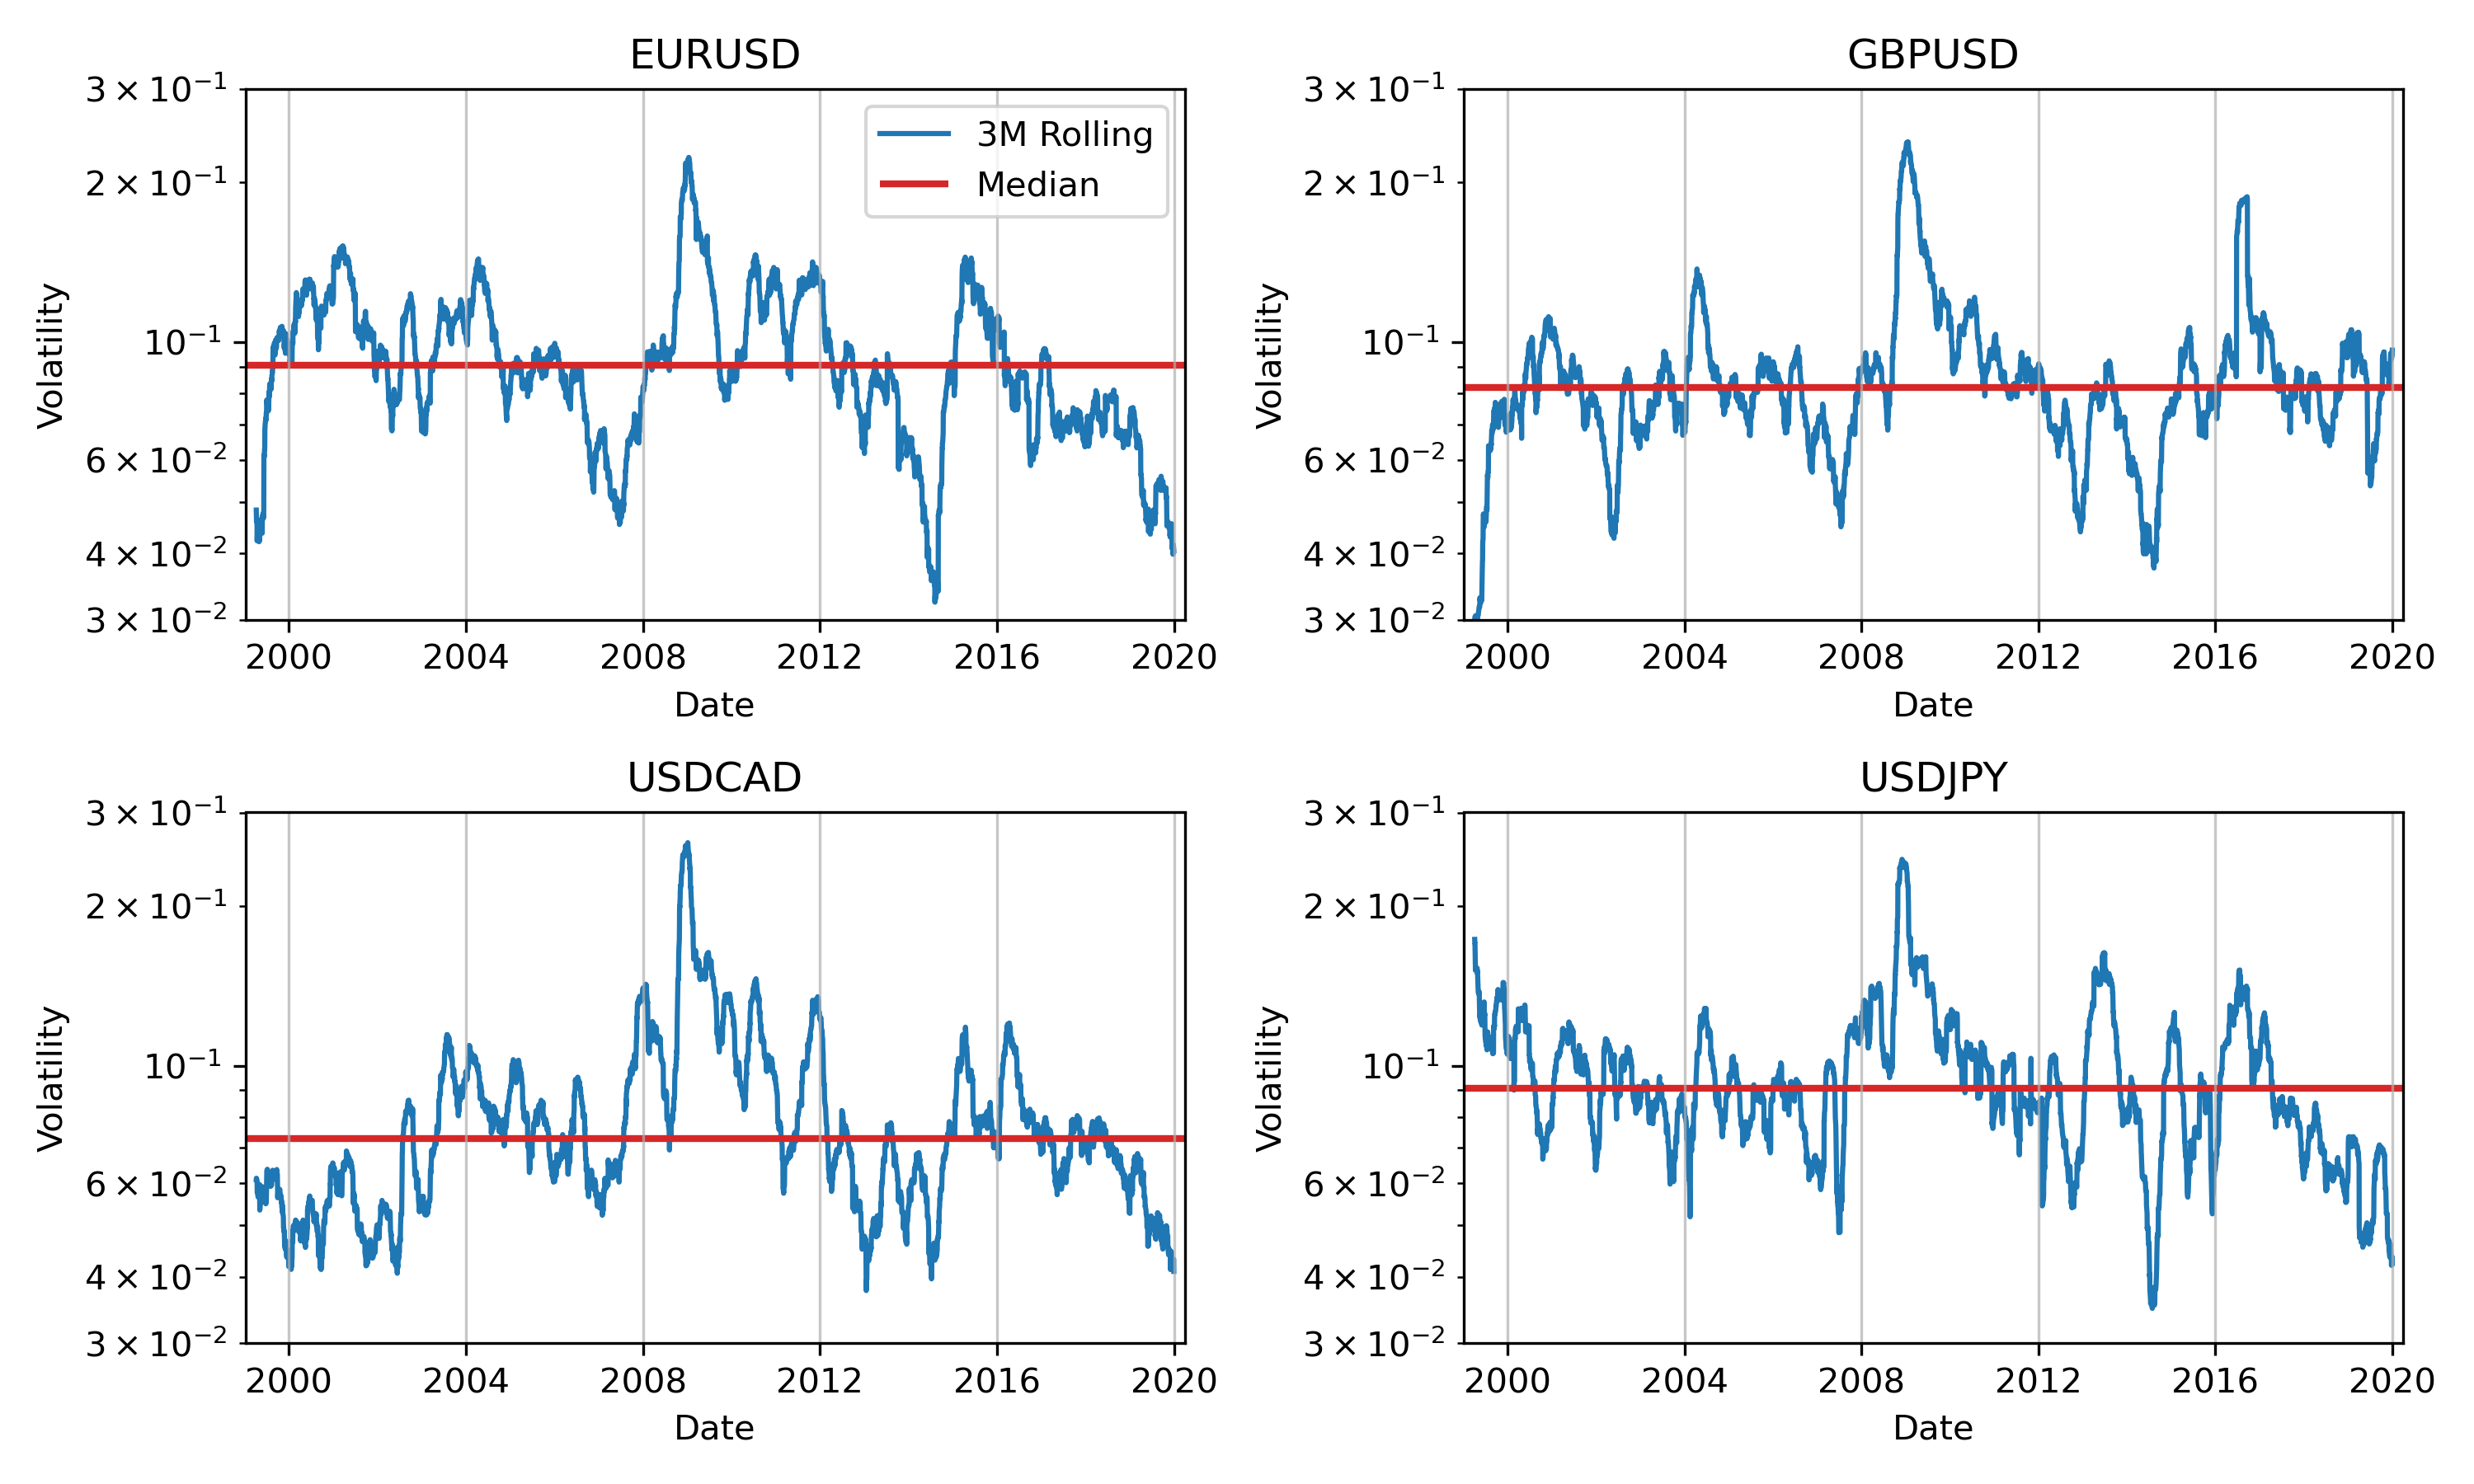
\includegraphics[width=1\linewidth]{data_analysis/rolling_volatility.png}
    \end{center}
    \caption{3-month rolling volatilities of the log returns data set compared to their historical medians.}
    \label{fig:rolling_volatility}
\end{figure}
